\documentclass[9pt, aspectratio=169]{beamer}
\usepackage{FiraSans}
\usetheme[subsectionpage=progressbar]{metropolis}
\usepackage[utf8]{inputenc}
\usepackage{amsmath}
\usepackage{amsfonts}
\usepackage{amssymb}
\usepackage{multicol}
\usepackage{tikz}
\usetikzlibrary{matrix}
\usepackage{caption}
\usepackage{xcolor}
\usepackage[T1]{fontenc} 
\usepackage[skins]{tcolorbox}
\author{Nicola Roman\`o - nicola.romano@ed.ac.uk}
\title{Lecture 11 - Convolutional Neural Networks (CNN)}
\setlength{\fboxsep}{0pt}
\setbeamertemplate {footline}{\begin{scriptsize}\hfill\insertframenumber ~of \inserttotalframenumber\kern1em\vskip5pt\end{scriptsize}}

% Remove "Figure" in front of captions
% See https://tex.stackexchange.com/questions/82456/how-to-remove-figure-caption-prefix-figure-in-beamer
\captionsetup{labelformat=empty,labelsep=none}

\titlegraphic{\centering \includegraphics[scale=.5]{instituteLogo.png}}
\date{}

\begin{document}

\newtcolorbox{codebox}{enhanced,
    top=2pt,
    left=2pt,
    right=2pt,
    bottom=2pt,
    boxrule=0pt,
    leftrule=5pt,
    sharp corners,
    colback=gray!20,
    colframe=blue!60!black}

\begin{frame}
    \titlepage
\end{frame}

\begin{frame}
    {Learning objectives}
    \begin{columns}
        \begin{column}{0.8\textwidth}
            \begin{itemize}
                \item LO 1
                \item LO 2
                \item LO 3
            \end{itemize}
        \end{column}
        \begin{column}{0.2\textwidth}
            
\includegraphics[angle=-30, origin=tr, width=1.5\textwidth]{lightbulb.png}
        \end{column}
    \end{columns}
\end{frame}

\section{Introduction}

\begin{frame}
    {From shallow to deep networks}
    In Lecture 11 we introduced neural networks. With increasing depth, neural networks can solve more complex problems.
    This comes at the cost of increased computational complexity (more parameters to learn).
    \vspace{1em}

    \begin{columns}[T]
        \begin{column}{.3\textwidth}
            \textbf{McCulloch-Pitts neuron}
            \vspace{2em}

            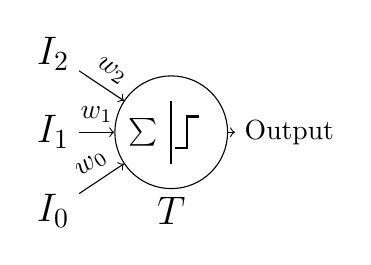
\begin{tikzpicture}[scale=1]
                % Neuron
                \node [draw, fill=white, circle, minimum height=4em] (n) at(1.5, 1) {$\sum\qquad$};
                \node [below of = n] {\Large\textbf{$T$}};

                % Inputs and weights
                \foreach \i in {0,1,2}
                    {
                        \node (i\i) at(0,\i) {\Large$I_\i$};
                        \draw [->] (i\i) -- node [above, midway, sloped] {\textbf{$w_\i$}} (n);
                    }

                \node (out) at(3, 1) {Output};
                \draw [->] (n) -- (out);
                \draw [thick] (1.5, .6) -- (1.5, 1.4);

                \draw [thick] (1.55, 0.8) -- (1.7, 0.8) -- (1.7, 1.2) -- (1.85, 1.2);
            \end{tikzpicture}
        \end{column}
        \begin{column}{.3\textwidth}
            \textbf{Single layer perceptron}
            \vspace{2em}

            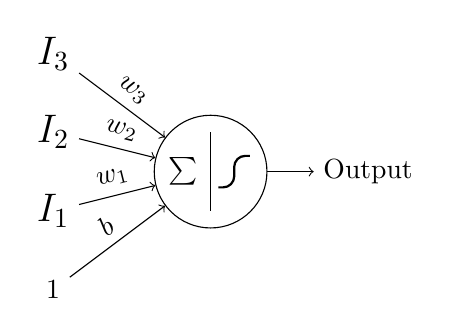
\begin{tikzpicture}
                % Neuron
                \node [draw, fill=white, circle, minimum height=4em] (n) at(2, 1.5) {$\sum\qquad$};

                % Bias
                \node (b) at(0, 0) {1};
                \draw [->] (b) -- node [above, midway, sloped] {\textbf{$b$}} (n);

                % Inputs and weights
                \foreach \i in {1,2,3}
                    {
                        \node (i\i) at(0,\i) {\Large$I_\i$};
                        \draw [->] (i\i) -- node [above, midway, sloped] {\textbf{$w_\i$}} (n);
                    }

                \node (out) at(4, 1.5) {Output};
                \draw [->] (n) -- (out);

                % Activation function
                \draw [thick, rounded corners] (2.1, 1.3) -- (2.3, 1.3) -- (2.3, 1.7) -- (2.5, 1.7);

                \draw (2, 1) -- (2, 2);
            \end{tikzpicture}
        \end{column}
        \begin{column}{.3\textwidth}
            \textbf{Multi-layer perceptron}
            \vspace{2em}

            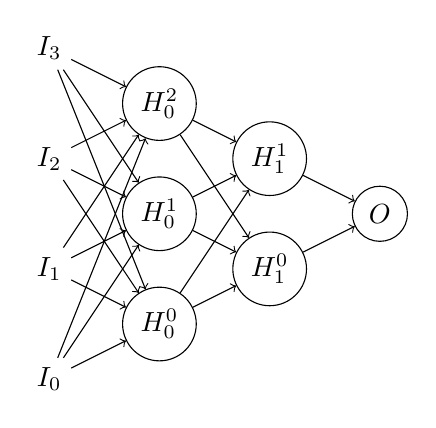
\begin{tikzpicture}[scale=.7]
                \tikzstyle{unit}=[draw,fill=white,shape=circle,minimum size=.7cm]

                \node (x0) at (0,0){$I_0$};
                \node (x1) at (0,2){$I_1$};
                \node (x2) at (0,4){$I_2$};
                \node (x3) at (0,6){$I_3$};

                \node[unit](h0) at (2,1){$H_0^0$};
                \node[unit](h1) at (2,3){$H_0^1$};
                \node[unit](h2) at (2,5){$H_0^2$};

                \node[unit](h3) at (4,2){$H_1^0$};
                \node[unit](h4) at (4,4){$H_1^1$};

                \node[unit](o) at (6,3){$O$};

                \draw[->] (x0) -- (h0);
                \draw[->] (x1) -- (h0);
                \draw[->] (x2) -- (h0);
                \draw[->] (x3) -- (h0);
                \draw[->] (x0) -- (h1);
                \draw[->] (x1) -- (h1);
                \draw[->] (x2) -- (h1);
                \draw[->] (x3) -- (h1);
                \draw[->] (x0) -- (h2);
                \draw[->] (x1) -- (h2);
                \draw[->] (x2) -- (h2);
                \draw[->] (x3) -- (h2);
                \draw[->] (h0) -- (h3);
                \draw[->] (h1) -- (h3);
                \draw[->] (h2) -- (h3);
                \draw[->] (h0) -- (h4);
                \draw[->] (h1) -- (h4);
                \draw[->] (h2) -- (h4);
                \draw[->] (h3) -- (o);
                \draw[->] (h4) -- (o);
            \end{tikzpicture}
        \end{column}
    \end{columns}

\end{frame}

\begin{frame}
    {Neural networks for image analysis}
    Can we use a MLP to analyze images?

    \begin{itemize}
        \item Input image: shape(w, h, c)
        \item Linearize image: shape(w x h x c)
        \item Use this vector as input to MLP
        \item Train and predict
    \end{itemize}

    Any problem with this?
    \pause

    \begin{itemize}[<+->]
        \item \textbf{It is impractical} for anything other than extremely small images.\\
              A small 256 x 256 RGB image gives 256 x 256 x 3 = 196608 inputs. Add a few hidden layers and the number of parameters to estimate becomes unmanageable.
        \item MLP are not \textbf{translation invariant}.\\
              If our network learns to detect a cell in the top-left part of the image, it won't be able to detect it in the bottom-right part.
        \item \textbf{We lose spatial information} when we flatten the image.\\
              Closeby pixels are more similar to each other than they are to the rest of the image. Problem for all other ML methods we have seen so far.
    \end{itemize}
\end{frame}

\begin{frame}
    {The solution?}
    \LARGE
    \centering
    Use convolutional filters!

    \normalsize
    (and have a neural network decide which to use!)
\end{frame}

\section{Convolutional filters}

\begin{frame}
    {Convolutional filters}
    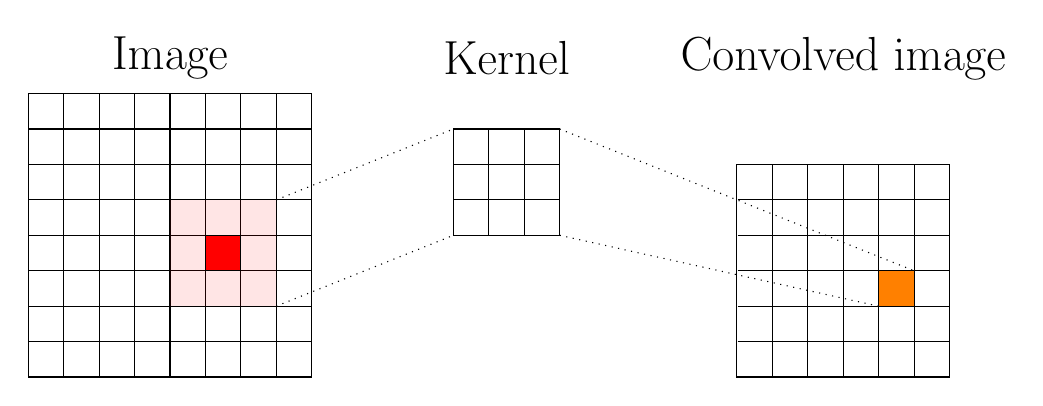
\begin{tikzpicture}[scale=.9]

        \draw [fill=white] (0, 0) rectangle (4, 4);
        \draw [step=0.5] (0.01, 0.01) grid (3.99, 3.99);
        \node at (2, 4.5) {\LARGE Image};

        \draw [fill=white] (6, 2) rectangle (7.5, 3.5);
        \draw [step=0.5] (6.01, 2.01) grid (7.49, 3.49);
        \node at (6.75, 4.5) {\LARGE Kernel};

        \draw [fill=red, opacity=0.1] (2, 1) rectangle (3.5, 2.5);
        \draw [fill=red] (2.5, 1.5) rectangle (3, 2);

        \draw [fill=white] (10, 0) rectangle (13, 3);
        \draw [step=0.5] (10.01, 0.01) grid (12.99, 2.99);
        \node at (11.5, 4.5) {\LARGE Convolved image};

        \draw [fill=orange] (12, 1) rectangle (12.5, 1.5);

        \draw [dotted] (3.5, 2.5) -- (6, 3.5);
        \draw [dotted] (3.5, 1) -- (6, 2);
        \draw [dotted] (7.5, 3.5) -- (12.5, 1.5);
        \draw [dotted] (7.5, 2) -- (12, 1);

    \end{tikzpicture}

    \LARGE
    $$O = \sum_i \sum_j I_{i,j} K_{i,j}$$

    \normalsize
    \begin{itemize}
        \item A 3x3 filter only has 9 parameters to learn, independently of image size.
        \item Convolutional filters are translation invariant.
        \item Convolution retains spatial information.
    \end{itemize}
    See Lecture 4 for a refresher.
\end{frame}

\begin{frame}
    {Some CNN convolution terminology}
    In CNN we define convolutional filters using:

    \begin{itemize}
        \item \textbf{Stride}: the number of pixels to skip between each filter application. Strides greater than 1 \textbf{reduce the size of the output}.
        \item \textbf{Padding}: the number of pixels to add to the input image to make it divisible by the filter size. Normally, zero-padding is used in CNN.
              \pause
        \item Some CNN terminology related to padding:
              begin{itemize}
        \item \textbf{Same padding}: we pad with the same amount of zeros on each side. If we use a stride of 1 we will have the same image shape after convolution.
        \item \textbf{Valide padding}: only \textbf{valid} data is used, meaning no padding. The output image is smaller than the input image, since we cannot process edge pixels.
    \end{itemize}
\end{frame}

\begin{frame}
    {Stride and padding - examples}
    \centering

    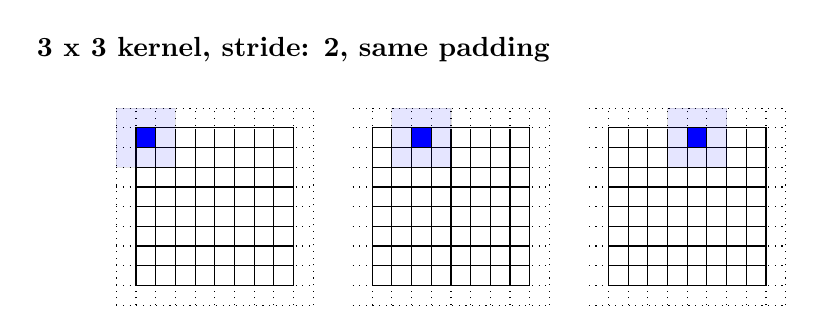
\begin{tikzpicture}
        \node at (2, 3) {\textbf{3 x 3 kernel, stride: 2, same padding}};

        \foreach \x [count=\step] in {0, 3, 6}
            {
                % Image
                \draw [fill=white] (\x, 0) rectangle (\x + 2, 2);
                \draw [fill=white, step=0.25] (\x+0.01, 0.01) grid (\x + 1.99, 1.99);
                % Padding
                \draw [dotted, step=0.25] (\x-0.25, -0.25) grid (\x + 2.25, 2.25);
                \draw [fill=blue, opacity=0.1] (\x + 0.5 * \step -0.75, 1.5) rectangle (\x + 0.5 * \step, 2.25);
                \draw [fill=blue] (\x + 0.5 * \step - 0.5, 1.75) rectangle (\x + 0.5 * \step -0.25, 2);
            }
    \end{tikzpicture}

    \pause

    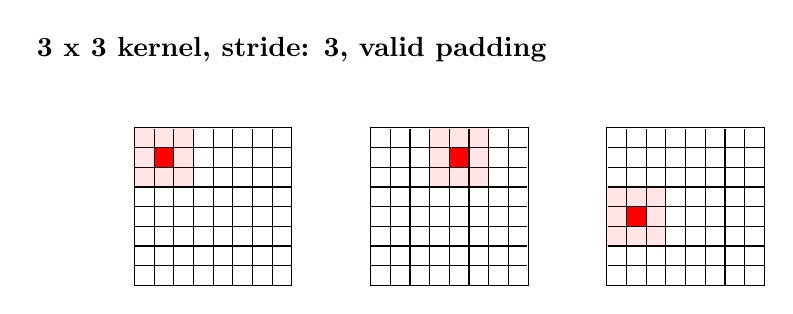
\begin{tikzpicture}
        \node at (2, 3) {\textbf{3 x 3 kernel, stride: 3, valid padding}};

        \foreach \x [count=\step] in {0, 3, 6}
            {
                % Image
                \draw [fill=white] (\x, 0) rectangle (\x + 2, 2);
                \draw [fill=white, step=0.25] (\x+0.01, 0.01) grid (\x + 1.99, 1.99);
            }
        \draw [fill=red, opacity=0.1] (0, 1.25) rectangle (0.75, 2);
        \draw [fill=red] (0.25, 1.5) rectangle (0.5, 1.75);
        \draw [fill=red, opacity=0.1] (3.75, 1.25) rectangle (4.5, 2);
        \draw [fill=red] (4, 1.5) rectangle (4.25, 1.75);
        \draw [fill=red, opacity=0.1] (6, 0.5) rectangle (6.75, 1.25);
        \draw [fill=red] (6.25, 0.75) rectangle (6.5, 1);
    \end{tikzpicture}
\end{frame}

\begin{frame}
    {Convolved image size}
    Given an image of size $n \times n$, a filter of size $k \times k$, stride $s$ and padding $p$ the output image size is:

    \Large
    $$\left\lfloor \frac{n + 2p - k}{s} + 1 \right\rfloor \times \left\lfloor \frac{n + 2p - k}{s} + 1 \right\rfloor$$
\end{frame}

\begin{frame}
    {Convolution of a volume}
    When applying convolution to a volume, we need to do it with a 3D filter.

    For example, we can convolve an RGB image with a $3\times 3\times 3$ filter.

    \begin{tikzpicture}
        \draw [fill=blue] (0.5, 0.5) rectangle (3.5, 3.5) grid [step=0.5] (0.5, 0.5);
        \draw [fill=green] (0.25, 0.25) rectangle (3.25, 3.25);
        \draw [step=0.5, shift={(0.25, 0.25)}] (0, 0) grid (3, 3);
        \draw [fill=red] (0, 0) rectangle (3, 3) grid [step=0.5] (0, 0);

        \node at (1.5, -1) {\LARGE $6\times 6$ RGB image};

        \draw [fill=teal!60!white, thick] (5.5, 2) rectangle (7, 3.5) grid [step=0.5] (5.5, 2);
        \draw [fill=teal!80!white, thick] (5.25, 1.75) rectangle (6.75, 3.25);
        \draw [step=0.5, shift={(0.25,0.25)}] (5, 1.5) grid (6.5, 3);
        \draw [fill=teal, thick] (5, 1.5) rectangle (6.5, 3) grid [step=0.5] (5, 1.5);

        \only<2>{
            \draw [fill=orange!60!white, thick] (5.5, 0) rectangle (7, 1.5) grid [step=0.5] (5.5, 0);
            \draw [fill=orange!80!white, thick] (5.25, -0.25) rectangle (6.75, 1.25);
            \draw [step=0.5, shift={(0.25,0.25)}] (5, -0.5) grid (6.5, 1);
            \draw [fill=orange, thick] (5, -0.5) rectangle (6.5, 1) grid [step=0.5] (5, -0.5);
        }
        \node at (4.2, 2) {\LARGE $\mathbf{\times}$};
        \only<1>{
            \node at (6, -1) {\LARGE $3\times 3\times 3$ filter};
        }
        \only<2>{
            \node at (6, -1) {\LARGE Two $3\times 3\times 3$ filters};
        }

        \node at (8, 2) {\LARGE $\mathbf{=}$};

        \only<1>{
            \draw [fill=teal] (9, 1) rectangle (11, 3) grid [step=0.5] (9, 1);
            \node at (10, -1) {\LARGE $4\times 4$ image};
        }
        \only<2>{
            \draw [fill=orange] (9.25, 1.25) rectangle (11.25, 3.25);
            \draw [step=0.5, shift={(0.25, 0.25)}] (9, 1) grid (11, 3);
            \draw [fill=teal] (9, 1) rectangle (11, 3) grid [step=0.5] (9, 1);
            \node at (10, -1) {\LARGE $4\times 4\times 2$ image};
        }
    \end{tikzpicture}
\end{frame}

\begin{frame}
    {Using convolution in an ANN}
    How can we make use of convolution in an ANN?

    The general idea behind convolutional neural networks

    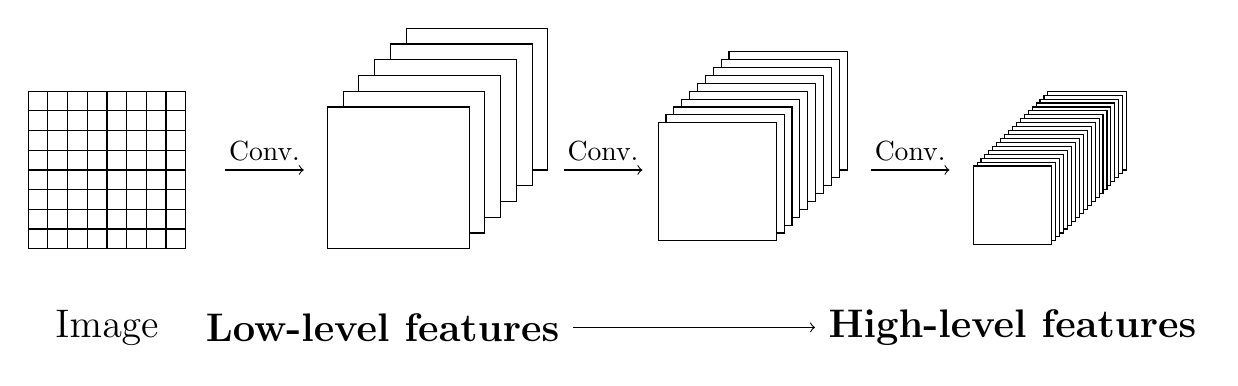
\begin{tikzpicture}
        \draw [fill=white] (0.5, 0) rectangle (2.5, 2);
        \draw [step=0.25] (0.51, 0.01) grid (2.49, 1.99);

        \foreach \z [count = \n] in {1, 0.8, ..., 0}
            {
                \draw [fill = white] (5.5 - \n * 0.2, \z) rectangle (7.3 - \n * 0.2, \z+1.8);
            }

        \foreach \z [count = \n] in {1, 0.9, ..., 0}
            {
                \draw [fill = white] (9.5 - \n * 0.1, \z) rectangle (11 - \n * 0.1, \z+1.5);
            }

        \foreach \z [count = \n] in {1, 0.95, ..., 0}
            {
                \draw [fill = white] (13.5 - \n * 0.05, \z) rectangle (14.5 - \n * 0.05, \z+1);
            }

        \draw [->] (3, 1) -- (4, 1) node [above, midway] {Conv.};
        \draw [->] (7.3, 1) -- (8.3, 1) node [above, midway] {Conv.};
        \draw [->] (11.2, 1) -- (12.2, 1) node [above, midway] {Conv.};

        \Large
        \node at (1.5, -1) {Image};
        \node (low) at (5, -1) {\textbf{Low-level features}};
        \node (high) at (13, -1) {\textbf{High-level features}};
        \draw [->] (low) -- (high);

    \end{tikzpicture}
\end{frame}

\section{Building a CNN}

\begin{frame}
    {Convolutional layers}

    \textbf{Convolutional layer}

    \begin{itemize}[<+->]
        \item Arguably the most important part of a CNN
        \item Performs a series of convolutions on the input image.
        \item Hyperparameters: number of convolutions, filter size, stride, padding.\\
              Note: the size, stride and padding are the same for all convolutions in the same layer.
        \item Parameters to learn: filter weights and biases.
        \item Number of parameters: $\text{num filters} \times \text{filter size}.$
        \item After convolution a non-linearity is introduced through the \textbf{activation function}. \textbf{ReLU} is the most commonly used.
    \end{itemize}

    \centering
    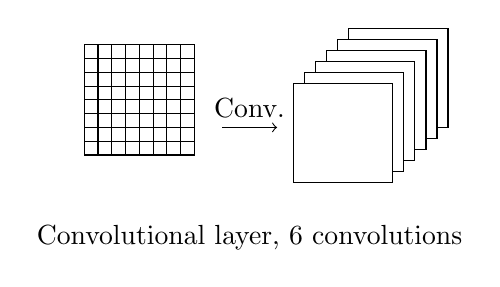
\begin{tikzpicture}[scale=0.7]
        \draw [fill=white] (0.5, 0.5) rectangle (2.5, 2.5);
        \draw [step=0.25] (0.51, 0.51) grid (2.49, 2.49);

        \foreach \z [count = \n] in {1, 0.8, ..., 0}
            {
                \draw [fill = white] (5.5 - \n * 0.2, \z) rectangle (7.3 - \n * 0.2, \z+1.8);
            }

        \draw [->] (3, 1) -- (4, 1) node [above, midway] {Conv.};

        \node at (3.5, -1) {Convolutional layer, 6 convolutions};
    \end{tikzpicture}
\end{frame}

\begin{frame}
    {Pooling layers - max pooling}
    \textbf{Max-pooling layer}

    \begin{itemize}[<+->]
        \item Performs a maximum filters on the input.
        \item Hyperparameters: filter size.
        \item Parameters to learn: none.
        \item Mostly used after a convolutional layer (thus some people call "convolutional + max pooling" a layer, others will consider them two layers, there is no consensus).
    \end{itemize}

    \centering
    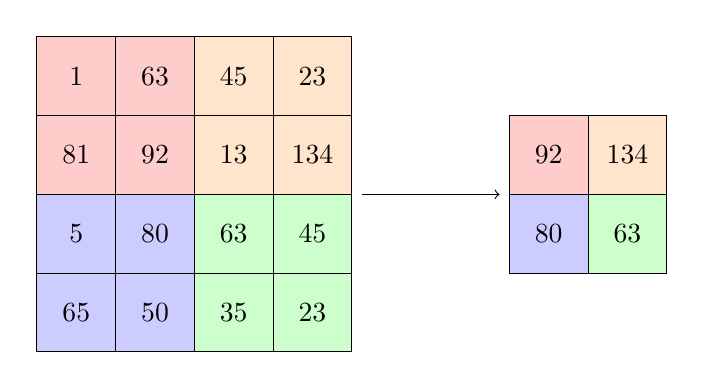
\begin{tikzpicture}
        \draw [fill=blue!20!white] (0, 0) rectangle (2, 2) grid (0, 0);
        \draw [fill=green!20!white] (2, 0) rectangle (4, 2) grid (2, 0);
        \draw [fill=red!20!white] (0, 2) rectangle (2, 4) grid (0, 2);
        \draw [fill=orange!20!white] (2, 2) rectangle (4, 4) grid (2, 2);

        \matrix (m) [matrix of nodes, ampersand replacement=\&, nodes={anchor=center, minimum width=1cm, minimum height = 1cm}] at (2, 2)
        {
            1 \& 63 \& 45 \& 23   \\
            81 \& 92 \& 13 \& 134 \\
            5 \& 80 \& 63 \& 45   \\
            65 \& 50 \& 35 \& 23  \\
        };

        \draw [fill=blue!20!white] (6, 1) rectangle (7, 2) grid (6, 1);
        \draw [fill=green!20!white] (7, 1) rectangle (8, 2) grid (7, 1);
        \draw [fill=red!20!white] (6, 2) rectangle (7, 3) grid (6, 2);
        \draw [fill=orange!20!white] (7, 2) rectangle (8, 3) grid (7, 2);

        \matrix (m1) [matrix of nodes, ampersand replacement=\&, nodes={anchor=center, minimum width=1cm, minimum height = 1cm}] at (7, 2)
        {
            92 \& 134 \\
            80 \& 63  \\
        };

        \draw [->] (m) -- (m1);
    \end{tikzpicture}
\end{frame}

\begin{frame}
    {Pooling layers - average pooling}
    \textbf{Average-pooling layer}

    \begin{itemize}[<+->]
        \item Performs average filtering on the input.
        \item Hyperparameters: filter size, stride.
        \item Parameters to learn: none.
        \item Rarely used nowadays
    \end{itemize}

    \centering

    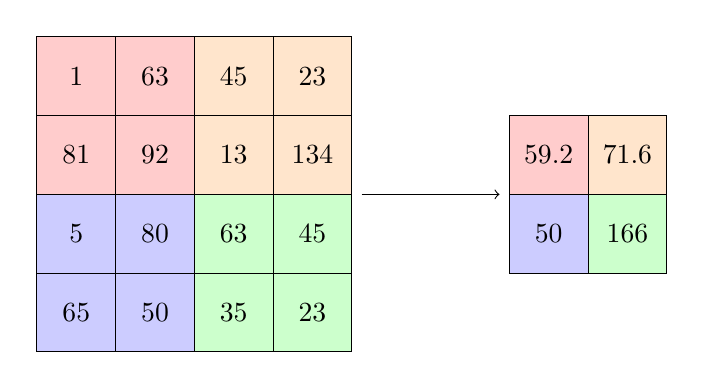
\begin{tikzpicture}
        \draw [fill=blue!20!white] (0, 0) rectangle (2, 2) grid (0, 0);
        \draw [fill=green!20!white] (2, 0) rectangle (4, 2) grid (2, 0);
        \draw [fill=red!20!white] (0, 2) rectangle (2, 4) grid (0, 2);
        \draw [fill=orange!20!white] (2, 2) rectangle (4, 4) grid (2, 2);

        \matrix (m) [matrix of nodes, ampersand replacement=\&, nodes={anchor=center, minimum width=1cm, minimum height = 1cm}] at (2, 2)
        {
            1 \& 63 \& 45 \& 23   \\
            81 \& 92 \& 13 \& 134 \\
            5 \& 80 \& 63 \& 45   \\
            65 \& 50 \& 35 \& 23  \\
        };

        \draw [fill=blue!20!white] (6, 1) rectangle (7, 2) grid (6, 1);
        \draw [fill=green!20!white] (7, 1) rectangle (8, 2) grid (7, 1);
        \draw [fill=red!20!white] (6, 2) rectangle (7, 3) grid (6, 2);
        \draw [fill=orange!20!white] (7, 2) rectangle (8, 3) grid (7, 2);

        \matrix (m1) [matrix of nodes, ampersand replacement=\&, nodes={anchor=center, minimum width=1cm, minimum height = 1cm}] at (7, 2)
        {
            59.2 \& 71.6 \\
            50 \& 166    \\
        };

        \draw [->] (m) -- (m1);
    \end{tikzpicture}

\end{frame}

\begin{frame}
    {After the convolutions - flatten and FC}
    Eventually, after all the convolutions we will need to flatten our output and feed it to a \textbf{fully-connected layer} (that is, a \textbf{multi-layer perceptron}!).

    This will take care, for example, of the final classification task.

    \centering
    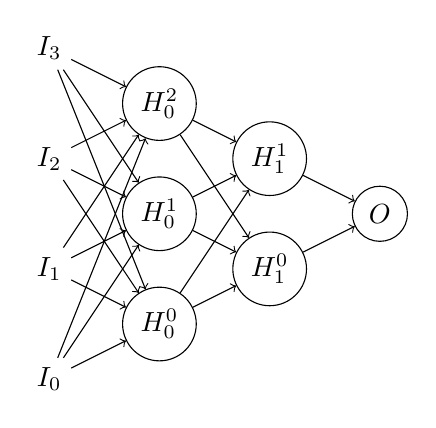
\begin{tikzpicture}[scale=.7]
        \tikzstyle{unit}=[draw,fill=white,shape=circle,minimum size=.7cm]

        \node (x0) at (0,0){$I_0$};
        \node (x1) at (0,2){$I_1$};
        \node (x2) at (0,4){$I_2$};
        \node (x3) at (0,6){$I_3$};

        \node[unit](h0) at (2,1){$H_0^0$};
        \node[unit](h1) at (2,3){$H_0^1$};
        \node[unit](h2) at (2,5){$H_0^2$};

        \node[unit](h3) at (4,2){$H_1^0$};
        \node[unit](h4) at (4,4){$H_1^1$};

        \node[unit](o) at (6,3){$O$};

        \draw[->] (x0) -- (h0);
        \draw[->] (x1) -- (h0);
        \draw[->] (x2) -- (h0);
        \draw[->] (x3) -- (h0);
        \draw[->] (x0) -- (h1);
        \draw[->] (x1) -- (h1);
        \draw[->] (x2) -- (h1);
        \draw[->] (x3) -- (h1);
        \draw[->] (x0) -- (h2);
        \draw[->] (x1) -- (h2);
        \draw[->] (x2) -- (h2);
        \draw[->] (x3) -- (h2);
        \draw[->] (h0) -- (h3);
        \draw[->] (h1) -- (h3);
        \draw[->] (h2) -- (h3);
        \draw[->] (h0) -- (h4);
        \draw[->] (h1) -- (h4);
        \draw[->] (h2) -- (h4);
        \draw[->] (h3) -- (o);
        \draw[->] (h4) -- (o);
    \end{tikzpicture}
\end{frame}

\begin{frame}
    {Putting it all together}
    We are now ready to put everything together.

    Example, we want to create a CNN that can classify an image as one of two classes (e.g. illness vs no illness).

    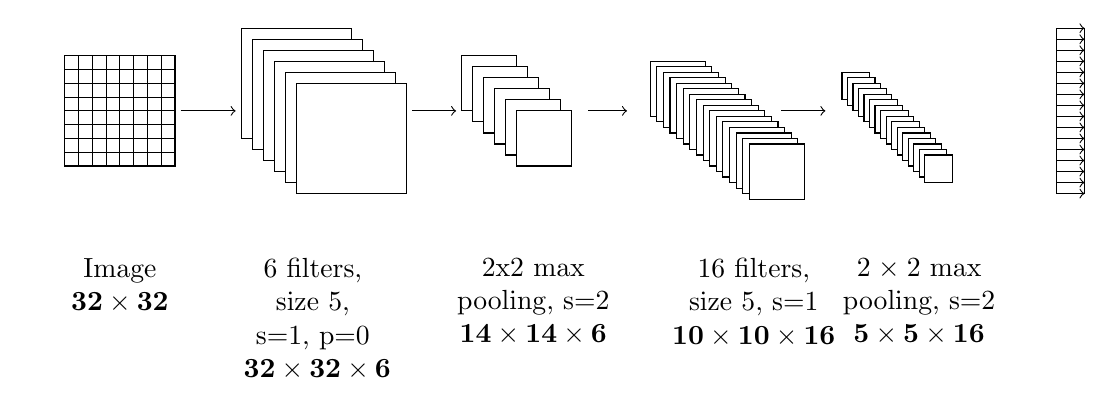
\begin{tikzpicture}[scale=0.7]
        \draw [fill=white] (0.5, 0.5) rectangle (2.5, 2.5);
        \draw [step=0.25] (0.51, 0.51) grid (2.49, 2.49);

        \node [text width=6em, align=center, anchor=north] at (1.5, -1) {Image $\mathbf{32\times 32}$};

        \draw [->] (2.6, 1.5) -- (3.6, 1.5);
        % Conv1
        \foreach \z [count = \n] in {1, 0.8, ..., 0}
            {
                \draw [fill = white] (3.5 + \n * 0.2, \z) rectangle (5.5 + \n * 0.2, \z+2);
            }

        \node [text width = 5em, align=center, anchor=north] at (5, -1) {6 filters, size 5, s=1, p=0 $\mathbf{32\times 32\times 6}$};

        \pause

        % Max pooling 1
        \draw [->] (6.8, 1.5) -- (7.6, 1.5);

        \foreach \z [count = \n] in {1, 0.8, ..., 0}
            {
                \draw [fill = white] (7.5 + \n * 0.2, \z + .5) rectangle (8.5 + \n * 0.2, \z+1.5);
            }


        \node [text width = 6em, align=center, anchor=north] at (9, -1) {2x2 max pooling, s=2 $\mathbf{14\times 14\times 6}$};

        \pause

        \draw [->] (10, 1.5) -- (10.7, 1.5);
        % Conv2
        \foreach \z [count = \n] in {1, 0.9, ..., -0.6}
            {
                \draw [fill = white] (11 + \n * 0.12, \z + .4) rectangle (12 + \n * 0.12, \z+1.4);
            }

        \node [text width = 6em, align=center, anchor=north] at (13, -1) {16 filters, size 5, s=1 $\mathbf{10\times 10\times 16}$};
        
        \pause 

        \draw [->] (13.5, 1.5) -- (14.3, 1.5);
        % Max pooling 2
        \foreach \z [count = \n] in {1, 0.9, ..., -0.6}
            {
                \draw [fill = white] (14.5 + \n * 0.1, \z + .7) rectangle (15 + \n * 0.1, \z+1.2);
            }

        \node [text width = 6em, align=center, anchor=north] at (16, -1) {$2\times 2$ max pooling, s=2 $\mathbf{5\times 5\times 16}$};

        \pause

        \draw [fill=white] (18.5, 0) rectangle (19, 3);
        \foreach \y in {3, 2.8, ..., 0}
            {
                \draw [->] (18.5, \y) -- (19, \y);
            }

    \end{tikzpicture}

\end{frame}

\end{document}

